
\appendix


\chapter{Data acquisition time stamps}
\label{app:A}
	
	\begin{table}[!htb]
		
		\centering
		\caption{Data acquisition timestamps.}
		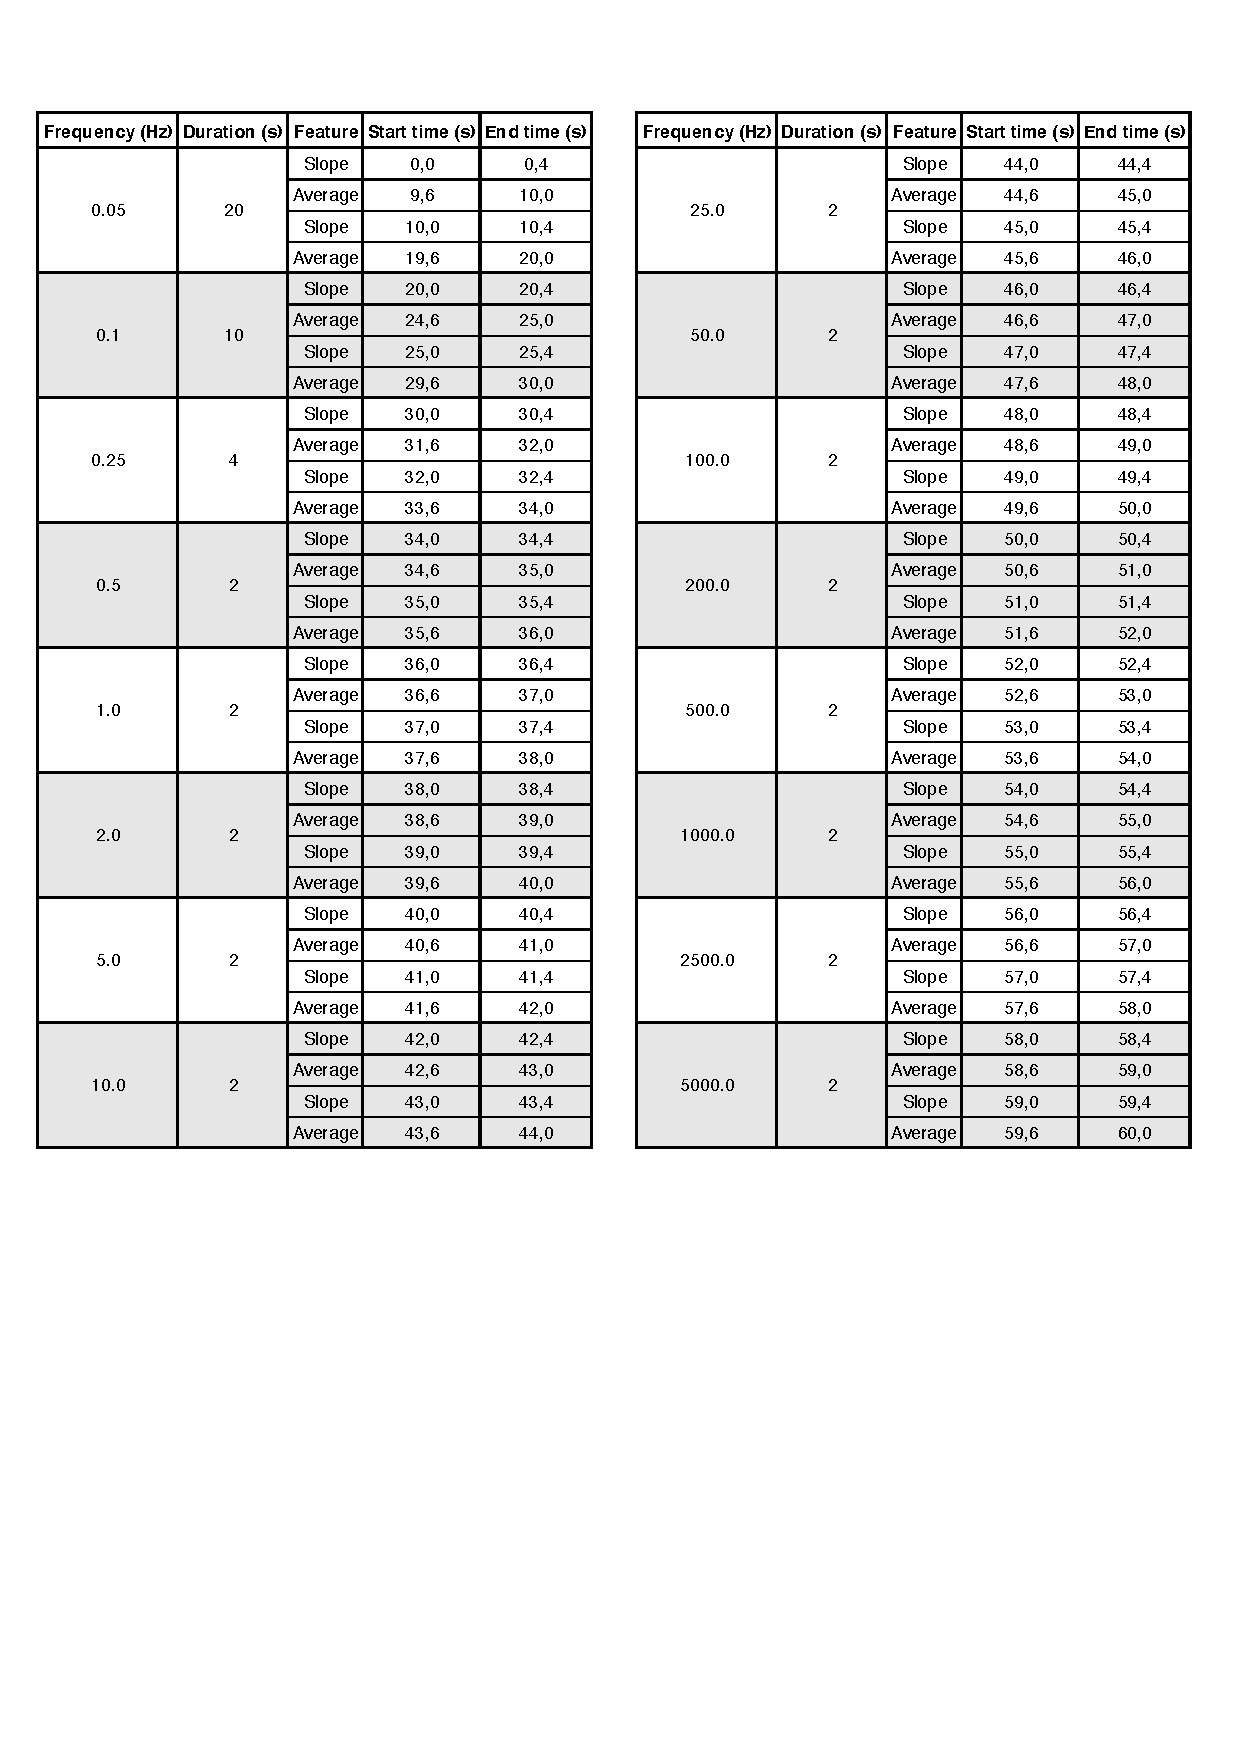
\includegraphics[width=0.7\textwidth]{../figures/timestamps.pdf}
		\label{fig:timestamps}
		
	\end{table}

\clearpage
\chapter{Other data plots}
\label{app:B}

\begin{figure}[!htb]
	\centering
	
	\begin{subfigure}[t]{1\textwidth}
		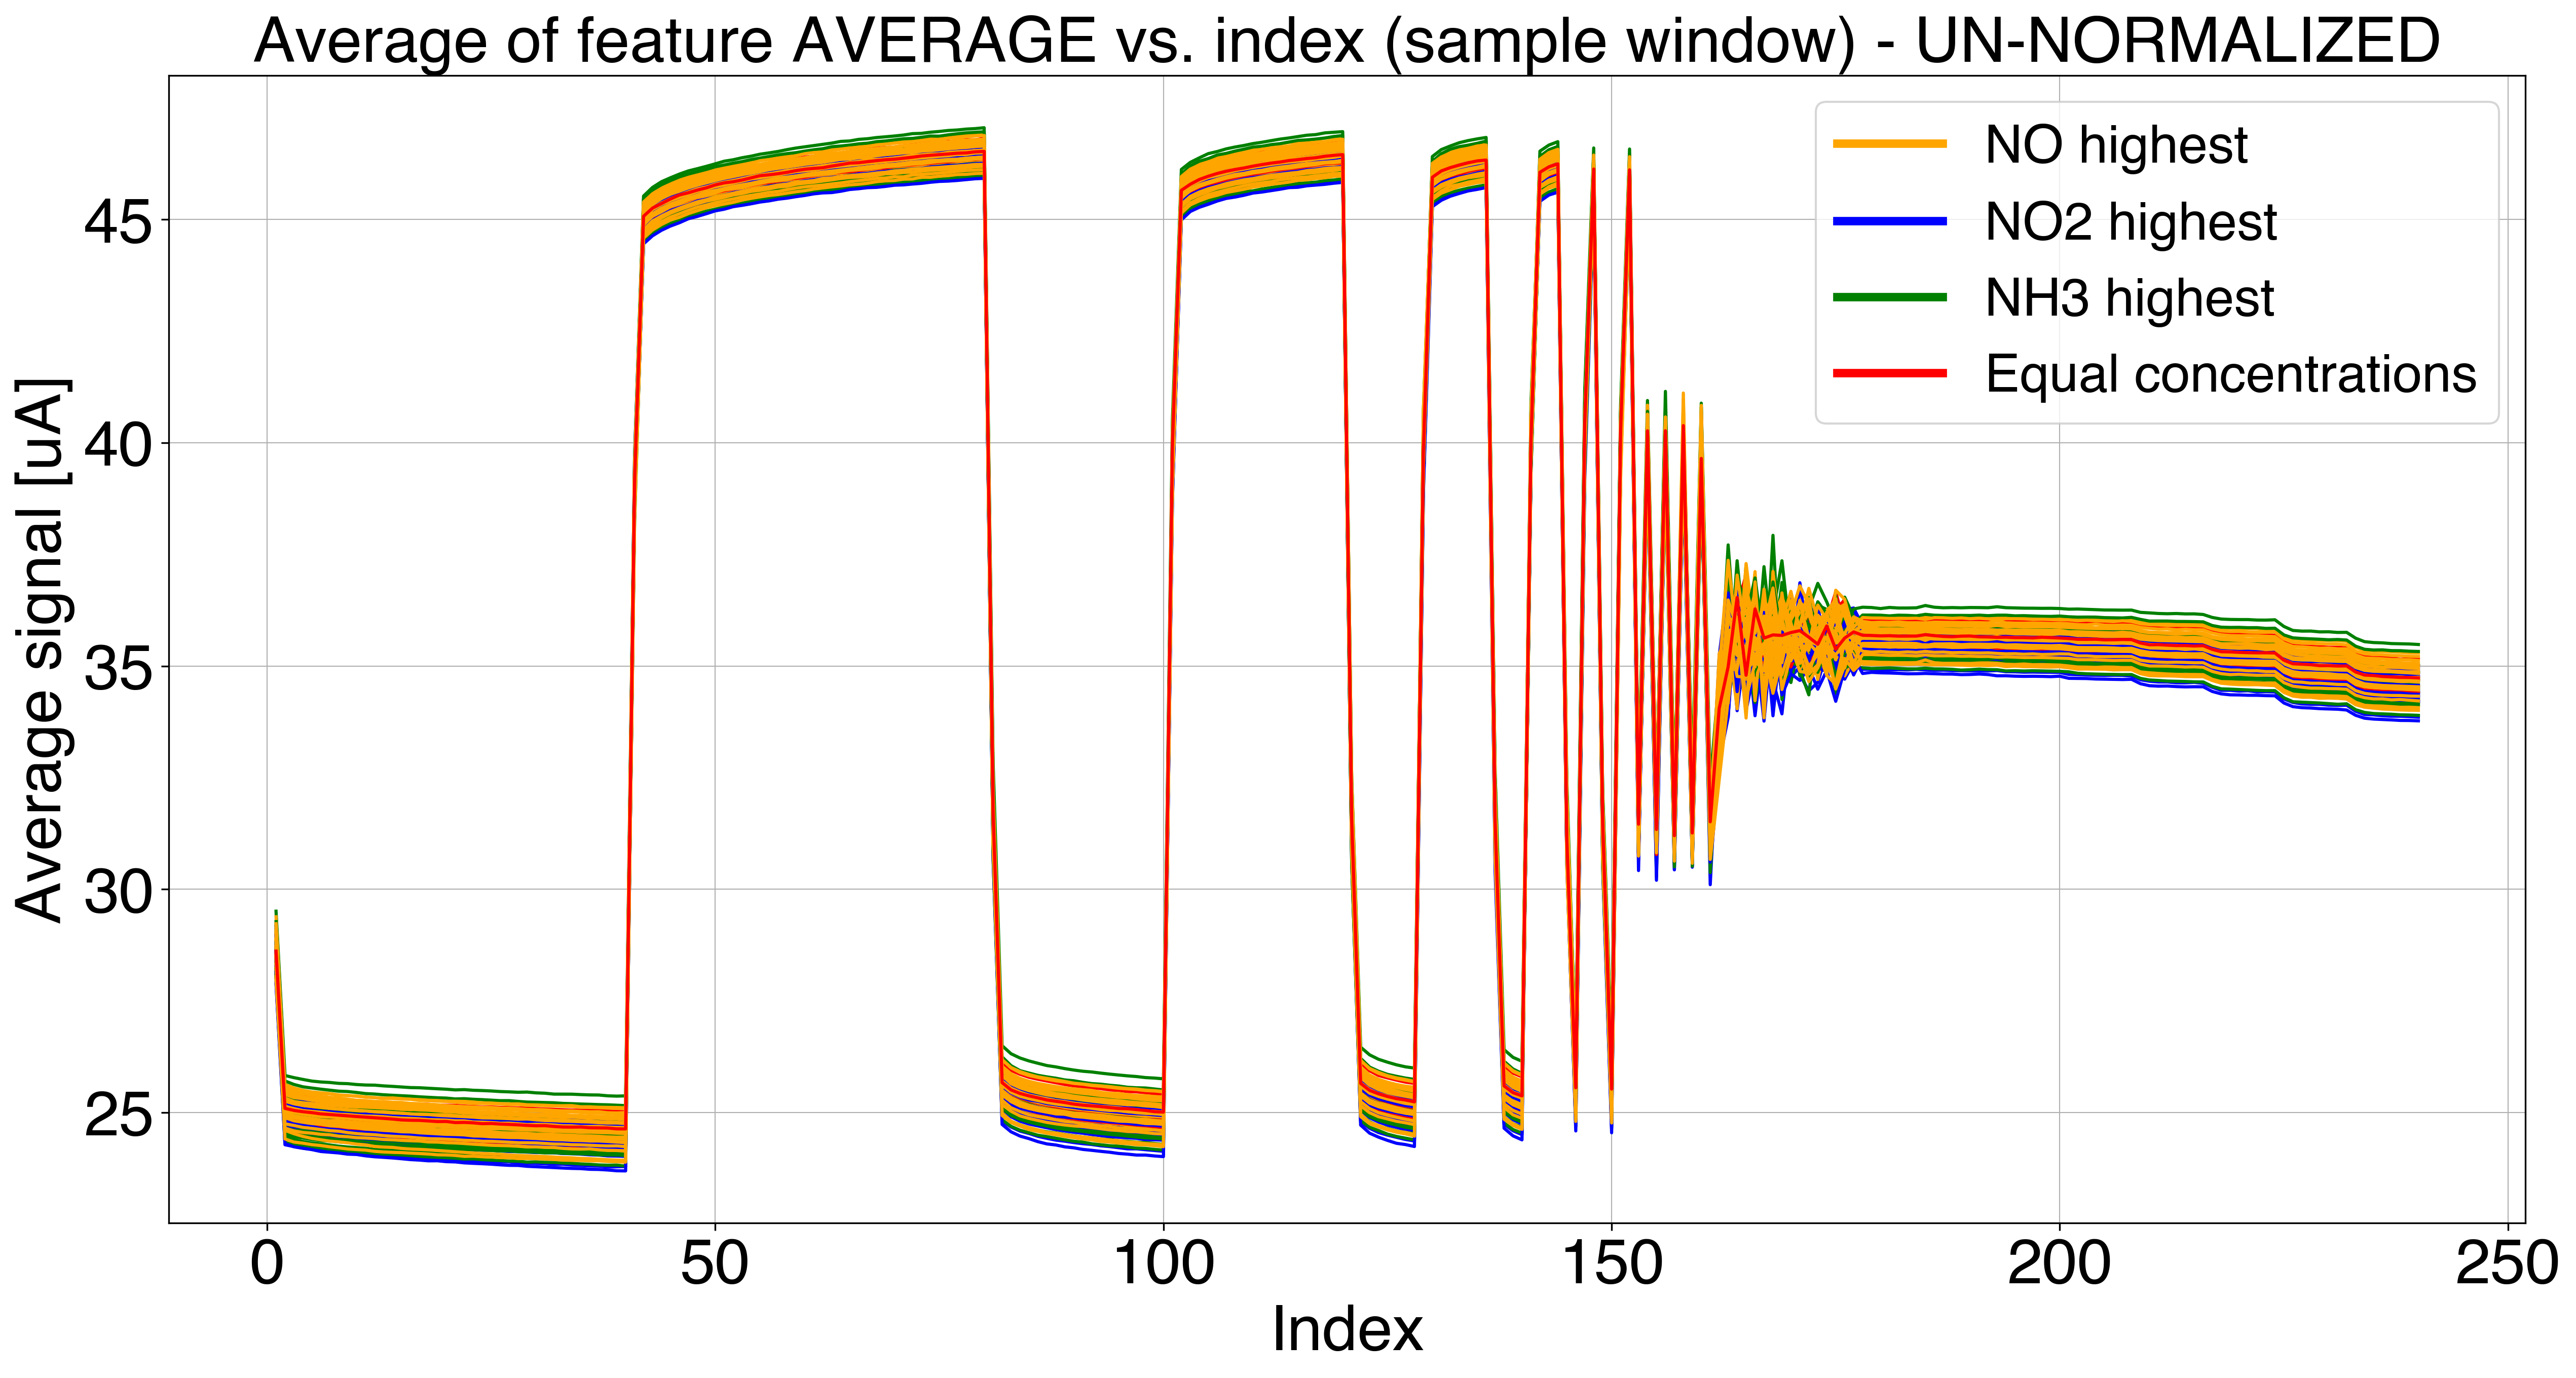
\includegraphics[width=1\linewidth]{../figures/order1.png}
		\caption{}
		\label{fig:order1} 
	\end{subfigure}
	
	\begin{subfigure}[t]{1\textwidth}
		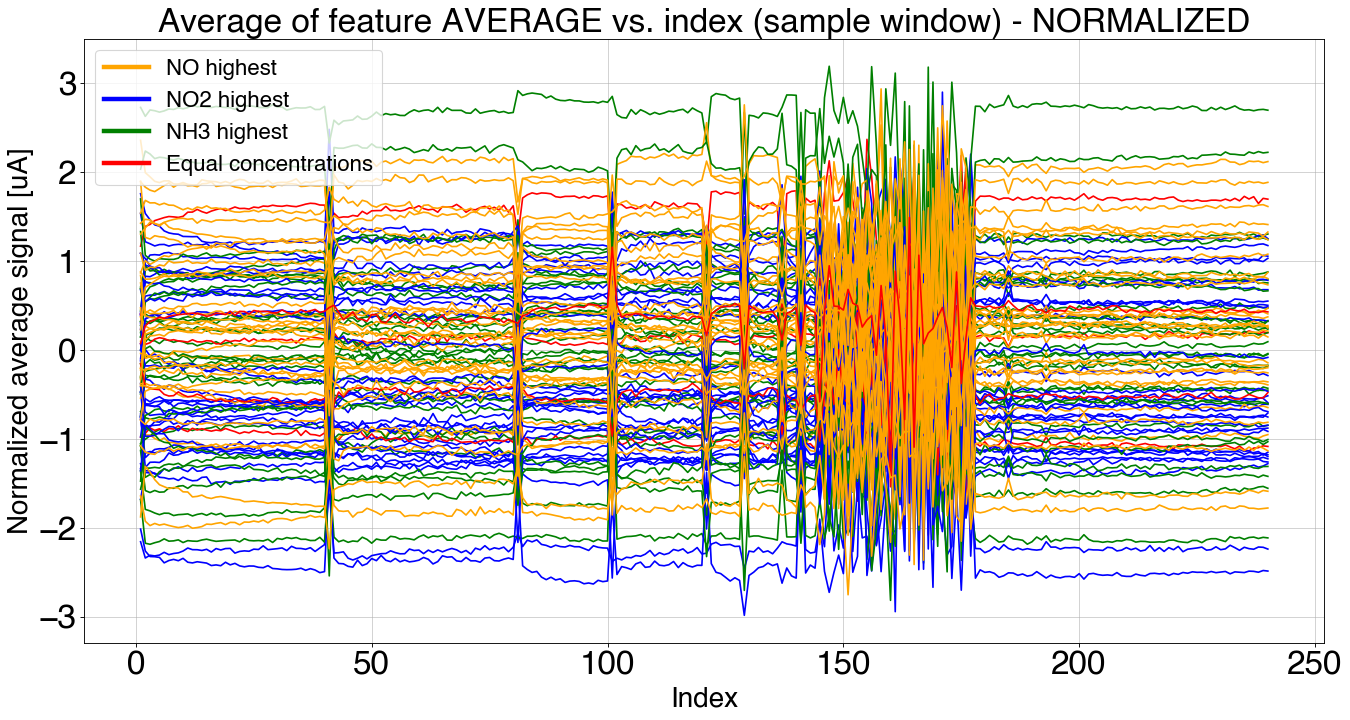
\includegraphics[width=1\linewidth]{../figures/order1-norm.png}
		\caption{}
		\label{fig:order1norm}
	\end{subfigure}
	
	\caption{Averaged sensor average divided by predominant gas. Each line corresponds to a unique mixture. }
	\label{fig:order1-both}
\end{figure}

\begin{figure}[!htb]
	\centering
	
	\begin{subfigure}[t]{0.9\textwidth}
		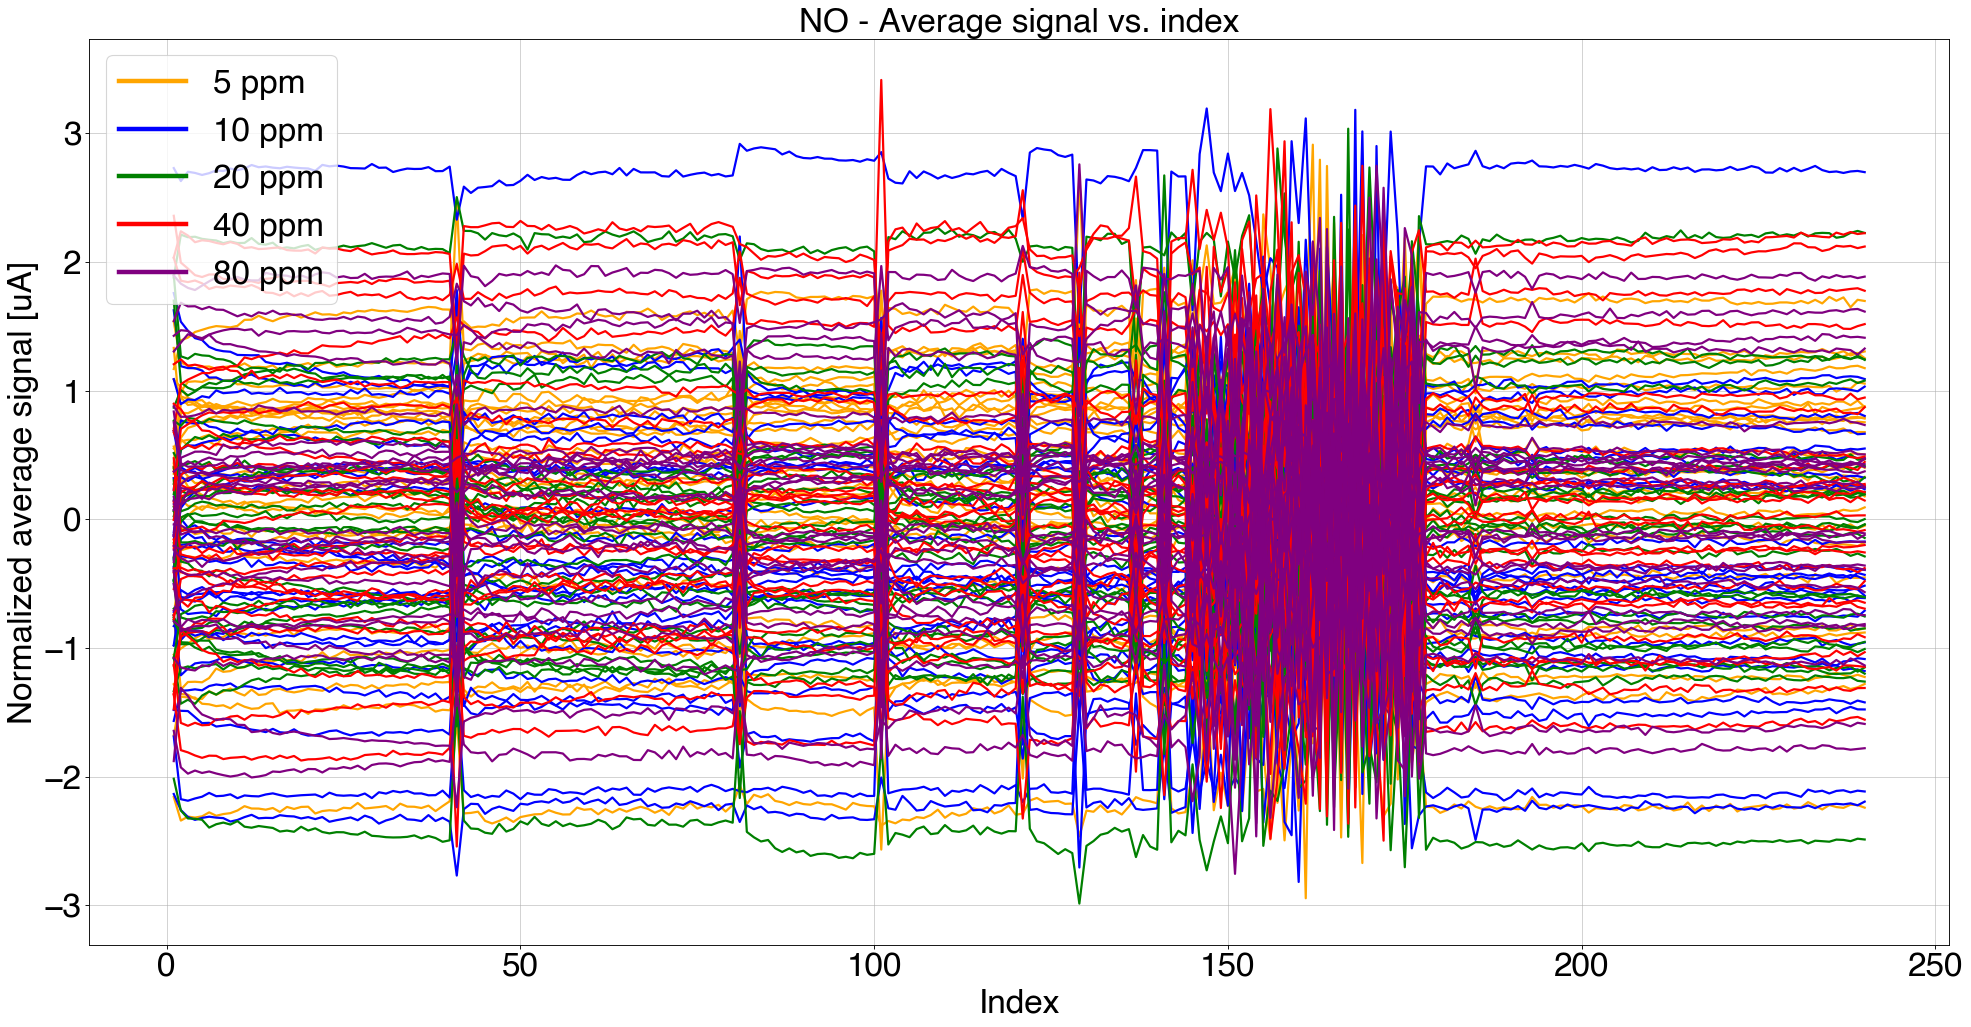
\includegraphics[width=1\linewidth]{../figures/order2NO.png}
		\caption{}
		\label{fig:order2NO} 
	\end{subfigure}
	
	\begin{subfigure}[t]{0.9\textwidth}
		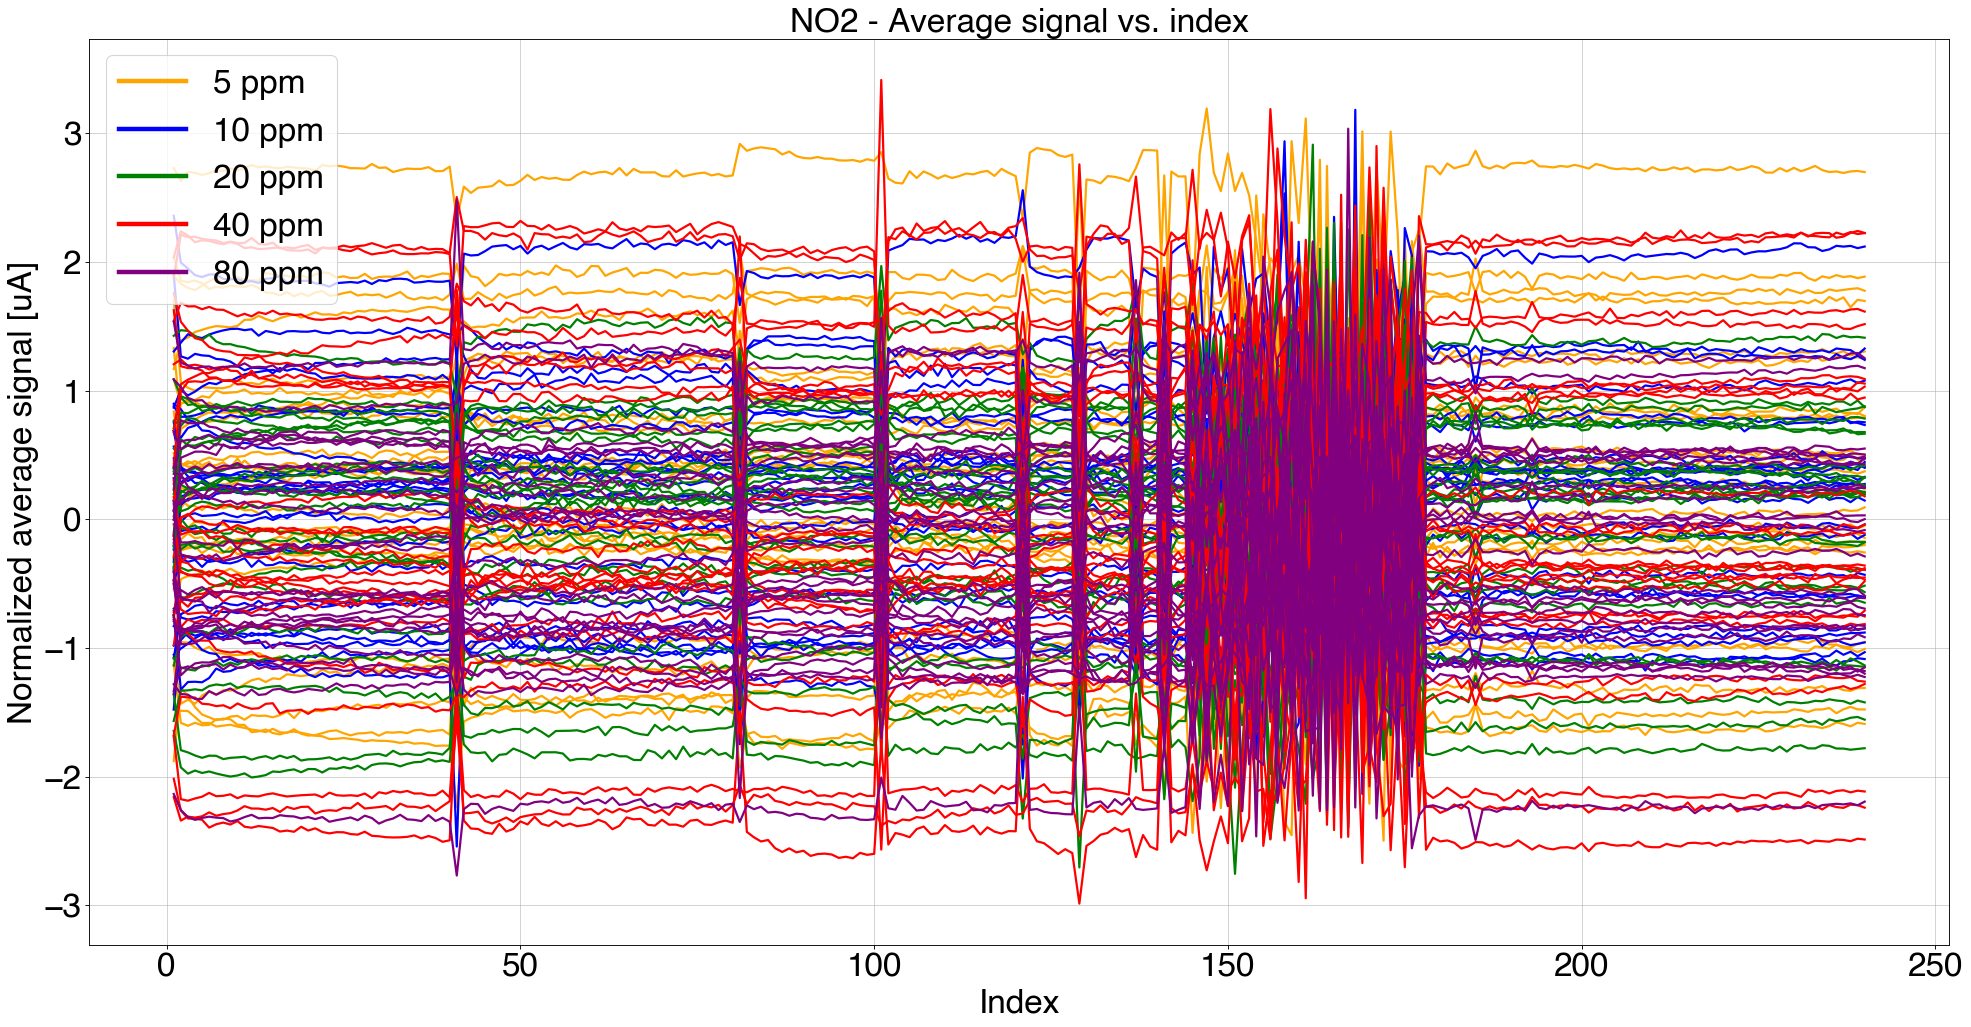
\includegraphics[width=1\linewidth]{../figures/order2NO2.png}
		\caption{}
		\label{fig:order2NO2}
	\end{subfigure}

	\begin{subfigure}[t]{0.9\textwidth}
		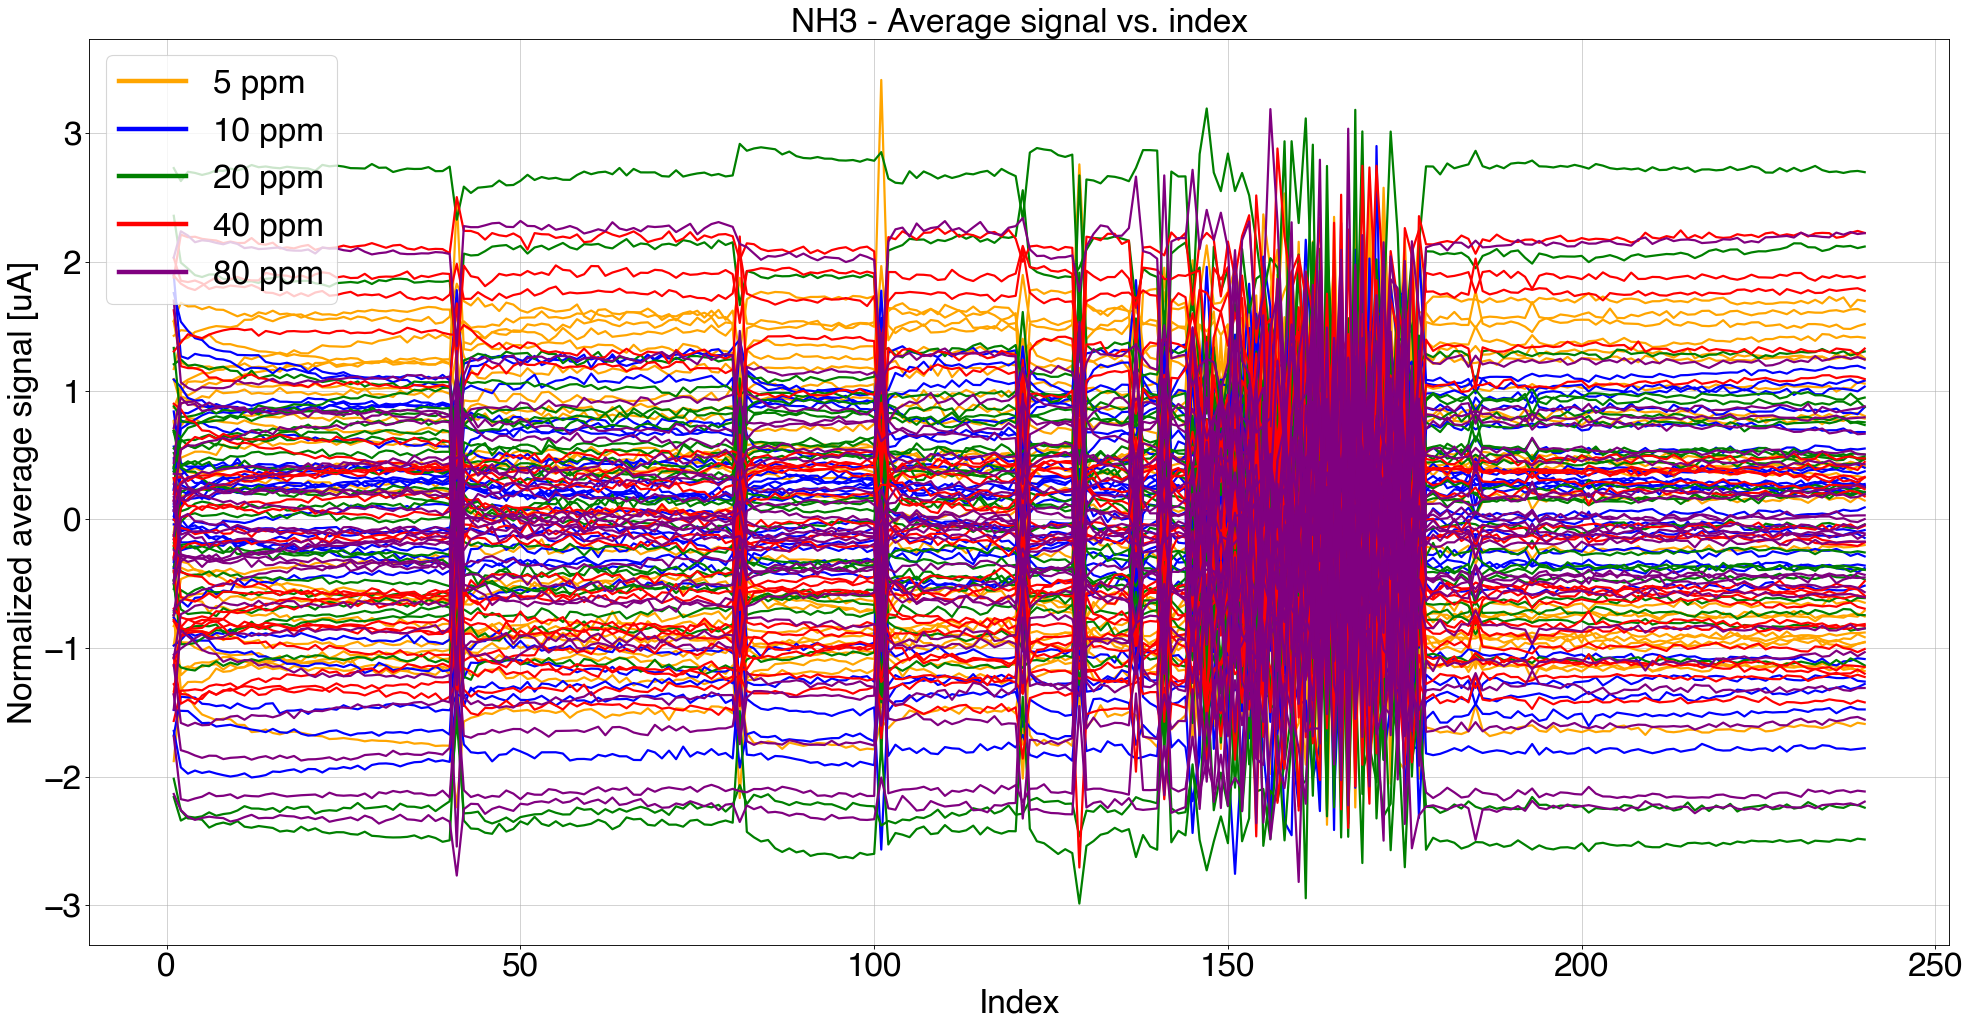
\includegraphics[width=1\linewidth]{../figures/order2NH3.png}
		\caption{}
		\label{fig:order2NH3}
	\end{subfigure}
	
	\caption{Normalized sensor averaged per gas. Each line corresponds to a unique mixture. The levels are the concentrations of individual components of the mixture: (a) NO (b) \ch{NO2}, and (c) \ch{NH3}}
	\label{fig:order2-both}
\end{figure}




